\chapter{Introduction}
This chapter provides the common thread of the work and positions it within the broader field of robotic manipulation and human-robot collaboration. 
First the \emph{Motivation} of the study is developed, followed by the \emph{Problem Description} and the resulting \emph{Aim of the Work}. 
Subsequent chapters present the \emph{State of the Art}, a formal \emph{Problem Statement}, the \emph{Related Work} and proposed methods, the experimental setup and evaluation, a discussion of the results
and their implications, and an outlook on future research directions.

    \section{Motivation}
    The motivation for this work is classified in a context and a use case, where the context outlines the growing role of industrial and collaborative manipulators,
    while the use case specifies a concrete manipulation scenario that requires accurate online identification of robot and payload parameters.

        \vspace{0.75\baselineskip}

        As the robotics industry grows year over year, so does the number of robots operating around the world. It is estimated that there were approximately 3.4 million industrial robots in use worldwide in
        2023~\cite{Q0_1_industrial_robots_in_operation}. At the same time, the number of newly installed industrial robots has been increasing steadily since 2014. Between 2021 and 2024, around 541\,000 new industrial
        robots were installed per year~\cite{Q0_2_industrial_robots_new_installations}. Within this landscape, collaborative robots (cobots) represent about 10.5\% of the industrial robot market, with 57\,040 new units 
        deployed in 2023, and annual cobot installations since 2020, 2022, and 2023 reaching roughly 50\,000 units per year. Importantly, these cobots are expected to complement rather than replace traditional industrial 
        robots~\cite{Q0_3_industrial_robots_new_cobot_installations_BarChart}.

        \begin{figure}[ht]
            \centering
            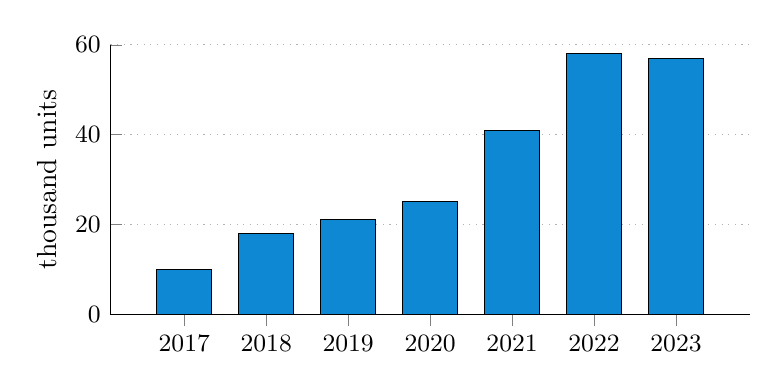
\begin{tikzpicture}
                \begin{axis}[
                        ybar,
                        bar width=20pt,
                        ymin=0, ymax=60,
                        width=0.8\linewidth,
                        height=5cm,
                        enlarge x limits=0.15,
                        axis x line*=bottom,
                        axis y line*=left,
                        ymajorgrids=true,
                        grid style={dotted,gray!60},
                        ylabel={thousand units},
                        xtick=data,
                        xticklabels={2017,2018,2019,2020,2021,2022,2023},
                        tick label style={font=\small},
                    ]
                    \addplot[fill=cyan!70!blue] coordinates {
                            (1,10)  % 2017
                            (2,18)  % 2018
                            (3,21)  % 2019
                            (4,25)  % 2020
                            (5,41)  % 2021
                            (6,58)  % 2022
                            (7,57)  % 2023
                        };
                \end{axis}
            \end{tikzpicture}
            \caption{Global annual installations of collaborative robots from 2017 to 2023 (in thousand units). Figure modified from~\cite{Q0_3_industrial_robots_new_cobot_installations_BarChart}.}\label{fig:cobot_installations}
        \end{figure}

        The growing deployment of, and increasing collaboration with, robots imposes stringent requirements on safety and performance. 
        As tasks become more complex and humans and robots share workspaces more closely, two closely related problems become central: 
        safe manipulation of payloads and safe physical human-robot interaction \cite{Q1_1_fast_inertial_id_cobots, Q1_2_online_payload_mo, Q1_5_payload_estimation_compensation_2025}. 
        Addressing both problems requires accurate knowledge of the inertial parameters of the manipulated object together with consistent estimation of
        the robot's dynamic state and interaction forces \cite{Q1_3_external_torque_smo, Q1_14_long2022sliding_momentum_observer, Q1_11_wei_composite_filter, Q3_2_encoder_attention_payload}. 
        A collaborative robot must therefore maintain an internal representation of the mass-inertia properties of the payload or tool it manipulates and of the forces exchanged with its environment. 
        This dynamic awareness is a prerequisite for compliant, contact-rich behaviour and for precise, high-performance manipulation in close proximity to humans
        \cite{Q1_7_10947736, Q1_8_10944553, Q1_9_xu2022_double_weighting_payload_id, % chktex 2
        Q1_10_duan_payload_ftsensor, Q1_13_dynamic_model_id_swevers2007}.

        \vspace{0.75\baselineskip}

        The considerations above motivate a concrete use case in which a collaborative robotic arm must manipulate previously unseen objects in a shared workspace. 
        A vision system can provide geometric information such as shape and dimensions of the payload, but it does not directly reveal its mass, center of mass (CoM), or inertia tensor. 
        For safe and precise execution of contact-rich tasks, however, these inertial properties are indispensable.

        In practice, the only viable way to obtain this information during operation is to exploit the robot's own sensor data, such as joint positions, velocities and accelerations, motor currents/torques,
        and optionally wrist force/torque measurements. 
        From these signals, one can estimate both the robot's rigid-body parameters and the inertial properties of the attached payload. 
        This leads to the dual identification problem of \emph{robot dynamic parameter identification} (RDPI) and \emph{payload dynamic parameter identification} (PDPI).

        The targeted application scenario comprises typical industrial and collaborative tasks such as pick-and-place, human-assisted manipulation, and precise tool use. 
        In all these cases, RDPI and PDPI must be performed online so that the controller maintains an up-to-date model of the combined robot-payload dynamics and the resulting contact forces. 
        Robust online identification methods are therefore a key enabling technology for safe human-robot collaboration and high-performance manipulation with arbitrary payloads and tools.

%%%%%%%%%%%%%%%%%%%%%%%%%%%%%%%%%%%%%%%%%%%%%%%%%%%%%%%%%%%%%%%%%%%%%%%%%%%%%%%%%%%%%%%%%%%%%%%%%%%%%%%%%%%%%%%%%%%%%%%%%%%%%%%%%%%%%%%%%%%%%%%%%%%%%%%%%%%%%%%%%%%%%%%%%%%%%%%%%%%%%%%%%%%%%%%%%%%%%%%%%%%%%%%%%%        
%%%%%%%%%%%%%%%%%%%%%%%%%%%%%%%%%%%%%%%%%%%%%%%%%%%%%%%%%%%%%%%%%%%%%%%%%%%%%%%%%%%%%%%%%%%%%%%%%%%%%%%%%%%%%%%%%%%%%%%%%%%%%%%%%%%%%%%%%%%%%%%%%%%%%%%%%%%%%%%%%%%%%%%%%%%%%%%%%%%%%%%%%%%%%%%%%%%%%%%%%%%%%%%%%%

    \section{Problem Description}
    The following kinematic and dynamic background of robot manipulation analyses why endowing a robotic manipulator with awareness of its own dynamics, payload, and tools is mathematically demanding and cannot be
    achieved by simple calculation or direct measurement alone.
        % ~\label{sec:robot_dynamics_background}
        The inertial properties of a rigid body are collected in the standard 10-dimensional parameter vector
        \begin{equation}
        \boldsymbol{\phi}^T
        =
        \begin{bmatrix}
            m & m c_x & m c_y & m c_z &
            J_{xx} & J_{xy} & J_{xz} & J_{yy} & J_{yz} & J_{zz}
        \end{bmatrix}
        \in \mathbb{R}^{10},
        \label{eq:rigidBody}
        \end{equation}
        which enters the Newton-Euler equations
        \begin{equation}
        \begin{bmatrix} 
            \mathbf{f} \\[2pt] \boldsymbol{\tau}
        \end{bmatrix}
        =
        m
        \begin{bmatrix}
            \mathbf{I}_{3\times3} & -[\mathbf{c}]^{\times} \\
            [\mathbf{c}]^{\times} & \mathbf{J}_s
        \end{bmatrix}
        \begin{bmatrix}
            \mathbf{a} \\[2pt] \boldsymbol{\alpha}
        \end{bmatrix}
        +
        \begin{bmatrix}
            m[\boldsymbol{\omega}]^{\times}[\boldsymbol{\omega}]^{\times}\mathbf{c} \\
            [\boldsymbol{\omega}]^{\times}\mathbf{J}_s\boldsymbol{\omega}
        \end{bmatrix},
        \label{eq:newtonEuler}
        \end{equation}
        so that the wrench $(\mathbf{f},\boldsymbol{\tau})$ depends nonlinearly on the motion $(\mathbf{a},\boldsymbol{\alpha},\boldsymbol{\omega})$ but linearly on $\boldsymbol{\phi}$.
        
        For the equipment rigidly attached to the tool flange (gripper/tool, with or without payload/load) we define an effective rigid-body parameter vector
        \begin{equation}
        \boldsymbol{\phi}_{\mathrm{eff}}
        =
        \begin{cases}
            \boldsymbol{\phi}_{\mathrm{tool}}, & \text{no load},\\[4pt]
            \boldsymbol{\phi}_{\mathrm{tool}} + \boldsymbol{\phi}_{\mathrm{load}}, & \text{with load},
        \end{cases}
        \label{eq:rigidEffective}
        \end{equation}
        which acts on top of the nominal robot dynamics. In contrast, with a clean flange (no tool/no load) only the robot parameters $\boldsymbol{\phi}_{\mathrm{robot}}$ contribute to the system dynamics.


        The robot structure itself is described by its own parameter vector $\boldsymbol{\phi}_{\mathrm{robot}}$, which enters the standard joint-space rigid-body dynamics. We denote this contribution by
        $\boldsymbol{\tau}_{\mathrm{robot}}$ (clean flange),
        \begin{equation}
        \boldsymbol{\tau}_{\mathrm{robot}}
        =
        \mathbf{M}(\mathbf{q}) \ddot{\mathbf{q}}
        +
        \mathbf{C}(\mathbf{q},\dot{\mathbf{q}})\dot{\mathbf{q}}
        +
        \mathbf{G}(\mathbf{q})
        +
        \boldsymbol{\tau}_f(\dot{\mathbf{q}}),
        \label{eq:robot_dynamics}
        \end{equation}
        where $\boldsymbol{\tau}_f(\dot{\mathbf{q}})$ models joint-level non-idealities such as Coulomb and viscous friction,
        possible Stribeck effects, and drive-train phenomena like backlash.
        
        The wrench generated by the effective rigid body at the flange induces an additional joint-space torque
        \begin{equation}
        \boldsymbol{\tau}_{\mathrm{ext}}
        =
        \mathbf{J}^T(\mathbf{q})\,\vec{F}_{\mathrm{ext}}(\boldsymbol{\phi}_{\mathrm{eff}}),
        \label{eq:tau_ext}
        \end{equation}
        where $\mathbf{J}(\mathbf{q})$ is the end-effector Jacobian. In the clean-flange case (no tool/no load), $\vec{F}_{\mathrm{ext}}$ reduces to purely external interaction forces with the environment (e.g.\ contacts or collisions).

    

        The motor torques are therefore
        \begin{equation}
        \boldsymbol{\tau}_{\mathrm{motor}}
        =
        \boldsymbol{\tau}_{\mathrm{robot}}
        +
        \boldsymbol{\tau}_{\mathrm{ext}}(\boldsymbol{\phi}_{\mathrm{eff}}),
        \label{eq:tau_motor}
        \end{equation}
        and for brushless DC actuators with torque constant $k_t$ one obtains the current-torque relation
        \begin{equation}
        \boldsymbol{\tau}_{\mathrm{motor}} = k_t\,\boldsymbol{I}
        \quad\Rightarrow\quad
        \boldsymbol{I}
        =
        \frac{\boldsymbol{\tau}_{\mathrm{robot}}
                + \boldsymbol{\tau}_{\mathrm{ext}}(\boldsymbol{\phi}_{\mathrm{eff}})}
            {k_t}.
        \label{eq:I_payload}
        \end{equation}

        If a force/torque sensor is mounted at the flange, the measured wrench can be written,
        using the relations derived in the Appendix~\ref{app:kinematic_background}, as
        \begin{equation}
        \vec{F}_{\mathrm{measured}}
        =
        Y\bigl(\mathbf{a},\boldsymbol{\alpha},\boldsymbol{\omega}\bigr)\,
        \boldsymbol{\phi}_{\mathrm{eff}}
        +
        \vec{F}_{\mathrm{bias}}
        +
        \vec{n},
        \label{eq:F_measured_regressor}
        \end{equation}

        where $Y(\cdot)$ is the $6\times 10$ Newton-Euler regressor matrix defined in the Appendix~\ref{app:query_categories}. It is linear in the inertial parameter vector $\boldsymbol{\phi}_{\mathrm{eff}}$, but depends nonlinearly on the motion variables $(\mathbf{a},\boldsymbol{\alpha},\boldsymbol{\omega})$. The terms $\vec{F}_{\mathrm{bias}}$ and $\vec{n}$ denote sensor bias and noise, respectively.
        The motion variables $(\mathbf{a},\boldsymbol{\alpha},\boldsymbol{\omega})$ are in turn determined by the joint state and motor torques through the nonlinear dynamics\eqref{eq:robot_dynamics}-\eqref{eq:I_payload}.

        From an identification viewpoint, this creates two tightly coupled challenges. 
        First, all available measurements (joint currents, positions, velocities and flange wrench) depend on the \emph{combined} dynamics of robot, tool and load via the nonlinear relationships~\eqref{eq:robot_dynamics}-\eqref{eq:F_measured_regressor}, so the contribution of the load parameters $\boldsymbol{\phi}_{\mathrm{load}}$ cannot be isolated by simple computation or direct measurement. 
        Second, accurate payload or load dynamic parameter identification (PDPI) presupposes an equally accurate compensation of the underlying robot-tool dynamics, including unmodelled effects such as friction and joint transmission nonlinearities. 
        Together, these aspects make dynamic awareness of payload, tool and robot a mathematically demanding inverse problem rather than a straightforward calculation from geometric or sensor data.

%%%%%%%%%%%%%%%%%%%%%%%%%%%%%%%%%%%%%%%%%%%%%%%%%%%%%%%%%%%%%%%%%%%%%%%%%%%%%%%%%%%%%%%%%%%%%%%%%%%%%%%%%%%%%%%%%%%%%%%%%%%%%%%%%%%%%%%%%%%%%%%%%%%%%%%%%%%%%%%%%%%%%%%%%%%%%%%%%%%%%%%%%%%%%%%%%%%%%%%%%%%%%%%%%%        
%%%%%%%%%%%%%%%%%%%%%%%%%%%%%%%%%%%%%%%%%%%%%%%%%%%%%%%%%%%%%%%%%%%%%%%%%%%%%%%%%%%%%%%%%%%%%%%%%%%%%%%%%%%%%%%%%%%%%%%%%%%%%%%%%%%%%%%%%%%%%%%%%%%%%%%%%%%%%%%%%%%%%%%%%%%%%%%%%%%%%%%%%%%%%%%%%%%%%%%%%%%%%%%%%%

        \section{Aim of Work}

        The SoA review highlights two persistent challenges for dynamic awareness in collaborative manipulation.
        First, accurate inverse-dynamics and friction compensation are often obtained in calibration-centric workflows that depend on carefully designed excitation and repeated identification runs.
        Second, hard-to-model effects (e.g., frictional memory and transmission nonlinearities) are frequently absorbed into lumped residual terms or task-specific models.
        Recent physics-informed architectures such as Deep Lagrangian Networks (DeLaN) provide a mechanics-consistent model class for inverse dynamics~\cite{Q4_2_lutter2023combiningphysicsdeeplearning,Q4_6_HU2026103093} and have been extended towards motor-side supervision when joint-torque measurements are unavailable~\cite{Q4_1_extended_delan_motor}.
        Complementarily, deep sequence models, in particular LSTMs, have been shown to be effective residual learners for dynamics and force/torque estimation from proprioceptive histories~\cite{Q3_1_tao_bll,Q3_3_lstm_force_estimation}.

        Aligned with the limitations identified in Chapter~2, the aim of this thesis is to develop and evaluate a \emph{physics-informed, sequence-model-based inverse-dynamics pipeline} that learns a single nominal actuation model from encoder and motor-current data, while separating structured rigid-body dynamics from history-dependent residual effects.
        This nominal model is intended to provide a foundation for tool/gripper compensation and subsequent payload dynamic parameter identification (PDPI) as formulated in Section~\ref{sec:robot_dynamics_background}.
        Although the structured inverse-dynamics formulation can, in principle, be interpreted in the end-effector wrench measurement frame via Jacobian mapping, the evaluation in this thesis is conducted purely in joint space in the measured actuation domain of motor currents.
        Concretely, the work pursues the following objectives:
        \begin{itemize}
        \item Learn a DeLaN-based baseline predictor of per-joint motor currents from joint kinematics, using a parameterisation that respects key mechanical structure (e.g., positive-definite inertia) and serves as a consistent nominal model~\cite{Q4_2_lutter2023combiningphysicsdeeplearning,Q4_6_HU2026103093}.
        \item Freeze the baseline and learn the remaining motor-current residual dynamics with an LSTM sequence model over a finite history window, capturing effects not explained by the instantaneous state alone~\cite{Q3_1_tao_bll,Q3_3_lstm_force_estimation}.
        \item Establish a trajectory-level split and model-selection protocol, and benchmark DeLaN and DeLaN+LSTM against the dataset baseline on the IEEE DataPort trajectories, reporting per-joint RMSE in current units [A]~\cite{Q_Dataset_Paper}.
        \end{itemize}

        Accordingly, the contributions of this work are a motor-current-domain formulation of a physics-structured DeLaN baseline. Combined with an LSTM residual model into a single inverse-dynamics predictor and an evaluation and best-model selection procedure, that quantifies accuracy and stability under trajectory-level splits. An implementation that reproduces preprocessing, training, and evaluation end-to-end within a containerised pipeline.

	        \begin{itemize}
	            \item[\textbf{RQ1}]
	                How accurately does a physics-structured DeLaN baseline predict per-joint motor currents on held-out trajectories, and how does trajectory coverage affect stability and generalisation (evaluated by per-joint motor-current RMSE in $\mathrm{A}$ on validation/test splits, reported as median $\pm$ IQR across seeds)?
	            \item[\textbf{RQ2}]
	                To what extent does an LSTM residual model reduce the remaining motor-current prediction error, and how do feature choice and history length influence accuracy and overfitting behaviour (evaluated by residual and combined motor-current RMSE in $\mathrm{A}$ on the test split, and by the overfit indicator $\mathcal{L}_{\mathrm{val}}/\mathcal{L}_{\mathrm{train}}$)?
	            \item[\textbf{RQ3}]
	                How does the proposed DeLaN+LSTM pipeline compare to the classical model-based identification baseline on the IEEE DataPort benchmark datasets and operating conditions~\cite{Q_Dataset_Paper} (evaluated by per-joint motor-current RMSE in $\mathrm{A}$ on the $5{,}000$-sample held-out test split and relative RMSE change versus the baseline)?
	        \end{itemize}
